% Options for packages loaded elsewhere
\PassOptionsToPackage{unicode}{hyperref}
\PassOptionsToPackage{hyphens}{url}
%
\documentclass[
  english,
  man]{apa6}
\usepackage{amsmath,amssymb}
\usepackage{lmodern}
\usepackage{ifxetex,ifluatex}
\ifnum 0\ifxetex 1\fi\ifluatex 1\fi=0 % if pdftex
  \usepackage[T1]{fontenc}
  \usepackage[utf8]{inputenc}
  \usepackage{textcomp} % provide euro and other symbols
\else % if luatex or xetex
  \usepackage{unicode-math}
  \defaultfontfeatures{Scale=MatchLowercase}
  \defaultfontfeatures[\rmfamily]{Ligatures=TeX,Scale=1}
\fi
% Use upquote if available, for straight quotes in verbatim environments
\IfFileExists{upquote.sty}{\usepackage{upquote}}{}
\IfFileExists{microtype.sty}{% use microtype if available
  \usepackage[]{microtype}
  \UseMicrotypeSet[protrusion]{basicmath} % disable protrusion for tt fonts
}{}
\makeatletter
\@ifundefined{KOMAClassName}{% if non-KOMA class
  \IfFileExists{parskip.sty}{%
    \usepackage{parskip}
  }{% else
    \setlength{\parindent}{0pt}
    \setlength{\parskip}{6pt plus 2pt minus 1pt}}
}{% if KOMA class
  \KOMAoptions{parskip=half}}
\makeatother
\usepackage{xcolor}
\IfFileExists{xurl.sty}{\usepackage{xurl}}{} % add URL line breaks if available
\IfFileExists{bookmark.sty}{\usepackage{bookmark}}{\usepackage{hyperref}}
\hypersetup{
  pdftitle={Temporal stability of idiographic psychological networks},
  pdfauthor={Ricarda K. K. Proppert1},
  pdflang={en-EN},
  hidelinks,
  pdfcreator={LaTeX via pandoc}}
\urlstyle{same} % disable monospaced font for URLs
\usepackage{graphicx}
\makeatletter
\def\maxwidth{\ifdim\Gin@nat@width>\linewidth\linewidth\else\Gin@nat@width\fi}
\def\maxheight{\ifdim\Gin@nat@height>\textheight\textheight\else\Gin@nat@height\fi}
\makeatother
% Scale images if necessary, so that they will not overflow the page
% margins by default, and it is still possible to overwrite the defaults
% using explicit options in \includegraphics[width, height, ...]{}
\setkeys{Gin}{width=\maxwidth,height=\maxheight,keepaspectratio}
% Set default figure placement to htbp
\makeatletter
\def\fps@figure{htbp}
\makeatother
\setlength{\emergencystretch}{3em} % prevent overfull lines
\providecommand{\tightlist}{%
  \setlength{\itemsep}{0pt}\setlength{\parskip}{0pt}}
\setcounter{secnumdepth}{-\maxdimen} % remove section numbering
% Make \paragraph and \subparagraph free-standing
\ifx\paragraph\undefined\else
  \let\oldparagraph\paragraph
  \renewcommand{\paragraph}[1]{\oldparagraph{#1}\mbox{}}
\fi
\ifx\subparagraph\undefined\else
  \let\oldsubparagraph\subparagraph
  \renewcommand{\subparagraph}[1]{\oldsubparagraph{#1}\mbox{}}
\fi
% Manuscript styling
\usepackage{upgreek}
\captionsetup{font=singlespacing,justification=justified}

% Table formatting
\usepackage{longtable}
\usepackage{lscape}
% \usepackage[counterclockwise]{rotating}   % Landscape page setup for large tables
\usepackage{multirow}		% Table styling
\usepackage{tabularx}		% Control Column width
\usepackage[flushleft]{threeparttable}	% Allows for three part tables with a specified notes section
\usepackage{threeparttablex}            % Lets threeparttable work with longtable

% Create new environments so endfloat can handle them
% \newenvironment{ltable}
%   {\begin{landscape}\begin{center}\begin{threeparttable}}
%   {\end{threeparttable}\end{center}\end{landscape}}
\newenvironment{lltable}{\begin{landscape}\begin{center}\begin{ThreePartTable}}{\end{ThreePartTable}\end{center}\end{landscape}}

% Enables adjusting longtable caption width to table width
% Solution found at http://golatex.de/longtable-mit-caption-so-breit-wie-die-tabelle-t15767.html
\makeatletter
\newcommand\LastLTentrywidth{1em}
\newlength\longtablewidth
\setlength{\longtablewidth}{1in}
\newcommand{\getlongtablewidth}{\begingroup \ifcsname LT@\roman{LT@tables}\endcsname \global\longtablewidth=0pt \renewcommand{\LT@entry}[2]{\global\advance\longtablewidth by ##2\relax\gdef\LastLTentrywidth{##2}}\@nameuse{LT@\roman{LT@tables}} \fi \endgroup}

% \setlength{\parindent}{0.5in}
% \setlength{\parskip}{0pt plus 0pt minus 0pt}

% Overwrite redefinition of paragraph and subparagraph by the default LaTeX template
% See https://github.com/crsh/papaja/issues/292
\makeatletter
\renewcommand{\paragraph}{\@startsection{paragraph}{4}{\parindent}%
  {0\baselineskip \@plus 0.2ex \@minus 0.2ex}%
  {-1em}%
  {\normalfont\normalsize\bfseries\itshape\typesectitle}}

\renewcommand{\subparagraph}[1]{\@startsection{subparagraph}{5}{1em}%
  {0\baselineskip \@plus 0.2ex \@minus 0.2ex}%
  {-\z@\relax}%
  {\normalfont\normalsize\itshape\hspace{\parindent}{#1}\textit{\addperi}}{\relax}}
\makeatother

% \usepackage{etoolbox}
\makeatletter
\patchcmd{\HyOrg@maketitle}
  {\section{\normalfont\normalsize\abstractname}}
  {\section*{\normalfont\normalsize\abstractname}}
  {}{\typeout{Failed to patch abstract.}}
\patchcmd{\HyOrg@maketitle}
  {\section{\protect\normalfont{\@title}}}
  {\section*{\protect\normalfont{\@title}}}
  {}{\typeout{Failed to patch title.}}
\makeatother
\shorttitle{Temporal stability idiographic networks}
\keywords{\newline\indent Word count: 000}
\DeclareDelayedFloatFlavor{ThreePartTable}{table}
\DeclareDelayedFloatFlavor{lltable}{table}
\DeclareDelayedFloatFlavor*{longtable}{table}
\makeatletter
\renewcommand{\efloat@iwrite}[1]{\immediate\expandafter\protected@write\csname efloat@post#1\endcsname{}}
\makeatother
\usepackage{lineno}

\linenumbers
\usepackage{csquotes}
\usepackage[titles]{tocloft}
\cftpagenumbersoff{figure}
\renewcommand{\cftfigpresnum}{\itshape\figurename\enspace}
\renewcommand{\cftfigaftersnum}{.\space}
\setlength{\cftfigindent}{0pt}
\setlength{\cftafterloftitleskip}{0pt}
\settowidth{\cftfignumwidth}{Figure 10.\qquad}
\cftpagenumbersoff{table}
\renewcommand{\cfttabpresnum}{\itshape\tablename\enspace}
\renewcommand{\cfttabaftersnum}{.\space}
\setlength{\cfttabindent}{0pt}
\setlength{\cftafterloftitleskip}{0pt}
\settowidth{\cfttabnumwidth}{Table 10.\qquad}
\ifxetex
  % Load polyglossia as late as possible: uses bidi with RTL langages (e.g. Hebrew, Arabic)
  \usepackage{polyglossia}
  \setmainlanguage[]{english}
\else
  \usepackage[main=english]{babel}
% get rid of language-specific shorthands (see #6817):
\let\LanguageShortHands\languageshorthands
\def\languageshorthands#1{}
\fi
\ifluatex
  \usepackage{selnolig}  % disable illegal ligatures
\fi
\newlength{\cslhangindent}
\setlength{\cslhangindent}{1.5em}
\newlength{\csllabelwidth}
\setlength{\csllabelwidth}{3em}
\newenvironment{CSLReferences}[2] % #1 hanging-ident, #2 entry spacing
 {% don't indent paragraphs
  \setlength{\parindent}{0pt}
  % turn on hanging indent if param 1 is 1
  \ifodd #1 \everypar{\setlength{\hangindent}{\cslhangindent}}\ignorespaces\fi
  % set entry spacing
  \ifnum #2 > 0
  \setlength{\parskip}{#2\baselineskip}
  \fi
 }%
 {}
\usepackage{calc}
\newcommand{\CSLBlock}[1]{#1\hfill\break}
\newcommand{\CSLLeftMargin}[1]{\parbox[t]{\csllabelwidth}{#1}}
\newcommand{\CSLRightInline}[1]{\parbox[t]{\linewidth - \csllabelwidth}{#1}\break}
\newcommand{\CSLIndent}[1]{\hspace{\cslhangindent}#1}

\title{Temporal stability of idiographic psychological networks}
\author{Ricarda K. K. Proppert\textsuperscript{1}}
\date{}


\note{s1348981}

\authornote{

Research Master thesis Clinical and Health Psychology, supervised by Dr.~Eiko Fried, Leiden University. Data and analysis script are available at Github.com/RicardaP/thesis\_repo.

Correspondence concerning this article should be addressed to Ricarda K. K. Proppert, . E-mail: \href{mailto:ricarda.proppert@gmail.com}{\nolinkurl{ricarda.proppert@gmail.com}}

}

\affiliation{\vspace{0.5cm}\textsuperscript{1} Leiden University, The Netherlands}

\abstract{
Evidence-based mental health programs have long conceptualized mental disorders in terms of interactions between thoughts, feelings, behaviours and external factors.

Idiographic network models are a relatively novel way of modeling such intra-individual psychological processes. These methods are not without limitations, and concerns have been raised about the stability and accuracy of estimated networks.

While methods to assess network parameter accuracy have been developed for cross-sectional data, no such method exists for single-subject data. The extend to which idiographic networks are stable, or vary over time, is unknown.

In the current work, we reanalyse daily symptom records of people with personality disorders to explore the stability of idiographic networks over time, as well as the degree to which network stability varies across individuals. We further explore antecents that may relate to inter-individual variation in network stability using predictive LASSO regression.
}



\begin{document}
\maketitle

\hypertarget{introduction}{%
\section{Introduction}\label{introduction}}

\hypertarget{idiographic-psychological-networks}{%
\subsection{Idiographic psychological networks}\label{idiographic-psychological-networks}}

Idiographic network models are of growing interest to clinical psychology because they may address two recently voiced calls in clinical psychology: First, there seems to be a need for psychological research to re-orient towards idiographic methods that study intra-individual processes as opposed to group-level differences (Molenaar, 2004).
Second, scholars have been proposing a paradigm shift away from reductionism towards studying the complexity of psychological phenomena.
The Network theory of mental disorders (Borsboom \& Cramer, 2013; Cramer, Waldorp, Maas, \& Borsboom, 2010) attempts to integrate psychology with insights and methods from complexity science, proposing a novel and well-received theoretical framework to study and understand the underpinnings of psychopathology.
The network theory of mental disorders conceptualizes psychopathology as an emergent state of dynamically interacting symptoms, as well as factors external to this system.
Importantly, it conceptualizes psychological symptoms as agents that contribute, not result from, psychopathology.
This account seems closely aligned with established clinical practices where informal case conceptualizations in form of path diagrams are used to describe the proposed mechanisms of a given disorder (Burger et al. (2020), Scholten, Lischetzke, and Glombiewski (2020)).

Psychological network models {[}@EpskampEtAl2018{]} are the methodological workhorse that quantify and visualize such system structures and dynamics.
Psychological network models consist of elements (nodes) and their pairwise interactions (edges), together representing a complex system.
Nodes typically represent psychological variables, e.g.~symptoms and behaviors, or influences from the external field, such as stressors.
Edges represent pairwise relationships between these variables.
These relationships may be directed or undirected , positive or negative, and can differ in strength.
Network models thus come in many different flavors, pertaining to the estimation procedures by which edge parameters are modeled and estimated, and lend themselves to a multitude of research questions.
As estimation procedures have been made readily available, the body of literature applying these methods is growing rapidly.
Most of the early psychological network research focused on comparing network structures across groups of people.
Recently, comparisons are also made within groups of people over time, for example, investigating the longitudinal network stability of PTSD symptoms in military veterans pre- to post-combat, Segal et al. (2020); during recovery, Stockert, Fried, Armour, and Pietrzak (2018); or in response to earthquake catastrophes, Ge, Yuan, Li, Zhang, and Zhang (2019).

\hypertarget{temporal-stability-of-networks}{%
\subsection{Temporal stability of networks}\label{temporal-stability-of-networks}}

Besides group-level analyses, there is growing interest in idiographic network models of intra-individual symptom dynamics.
Researchers in clinical psychology in particular hope that such models could resolve what is known as the Therapist's dilemma (eg., Frumkin, Piccirillo, Beck, Grossman, and Rodebaugh (2020), Howe, Bosley, and Fisher (2020), Caviglia and Coleman (2016), Hoffart and Johnson (2020)).
In clinical psychology research, not only momentary network structures are of interest, but especially \emph{changes} in network structure over time.
For example, changes in network structure may indicate therapeutic progress (Thonon, Van Aubel, Lafit, Della Libera, \& Larøi, 2020) or relapse (Wichers, Groot, \& Psychosystems, 2016).
Even subtle changes in network structure are of interest, as they are thought to act as potential early warning signals which may predict future major change, i.e.~a system's phase transition from a healthy attractor state to a disordered one.
For example, signs of critical slowing down, showing as increased auto-correlations and variances of items, have been demonstrated to signal a patient's relapse into depression upon stopping antidepressant treatment (Wichers, Groot, and Psychosystems (2016); for similar work on resilience, see Kuranova et al. (2020)).

Differences in network structures are often interpreted at face value.
For example, Thonon, Van Aubel, Lafit, Della Libera, and Larøi (2020) followed three psychiatric patients over the course of treatment and interpreted changes in idiographic network structures over time as additional evidence for and a description of the observed therapeutic change.
Such a substantial interpretation of network instability assumes that differences in estimated network parameters accurately reflect a change in the data-generating process.
This assumption rests on two conditions: First, parameter estimates need to be an accurate reflection of the true underlying relationship, meaning they should be unbiased and reliable.
Second, the underlying mechanism is assumed to have remained stable if no intervention took place.
Neither of these conditions can currently be evaluated for idiographic network models.
While bootstrapping procedures to assess the accuracy and reliability of parameter estimates have been developed for neworks estimated on group-level data (Epskamp, Borsboom, \& Fried, 2018), comparable tools are not yet available for idiographic estimation methods.
Furthermore, the degree to which complex psychological processes are stable within individuals over time is unclear.
Current literature investigating the temporal stability of idiographic networks mostly focuses on settings where change is expected to occur, e.g., in response to psychological treatment (Thonon, Van Aubel, Lafit, Della Libera, \& Larøi, 2020), discontinuation of antidepressant medication (Wichers, Groot, \& Psychosystems, 2016), or the COVID-19 pandemic (Emorie D. Beck \& Jackson, 2021).

To our knowledge, only one study has investigated the temporal stability of idiographic psychological networks in a setting where no profound change was expected.
Emorie D. Beck and Jackson (2020) investigated the consistency of idiographic personality over the course of two years.
Their study reports high consistency among contemporaneous associations, and low consistency of temporal associations.
Interestingly, they found considerable interpersonal variability in the stability of networks, which appeared to be weakly related to participants life satisfactions.

Summing up, psychological network models have been described as ``window into a patient's daily life'' Epskamp et al. (2018).
The question remains whether this window provides an unobstructed and representative view.
Is this window a doorhole, or a panorama front?
Are we getting a clear view inside, or are we mostly seeing our own reflections?

\hypertarget{conceptual-distinctions}{%
\subsection{Conceptual distinctions}\label{conceptual-distinctions}}

Recent reviews have raised concerns that the network approach may leave important methodological challenges unaddressed.
Most prominently, there appears to be disagreement on whether findings in the network literature are replicable or might propell psychologiy back into the replication crisis it is trying to recover from.
(CITE forbes und co).
We will briefly outline the most relevant methodological concepts that should be considered in relation to temporal network stability.
It should be noted that many of these concepts are not clearly distinguished in the current literature, and that terms tend to be used interchangeably.
In the current work, we strive to keep a consistent distinction, but the definitions applied here may not be accurate given the lack of agreement in current publications.

\hypertarget{network-theory-versus-network-models}{%
\subsubsection{Network theory versus network models}\label{network-theory-versus-network-models}}

Network theory \ldots{} Network models \ldots{} graphical Vector Autoregressive models / partial correlation models popular in idiographic research, but other estimation methods exist, which each their strengths and limitations.

\hypertarget{stability-of-complex-systems-vs-stability-of-network-models}{%
\subsubsection{Stability of complex systems vs stability of network models}\label{stability-of-complex-systems-vs-stability-of-network-models}}

Stabilitiy of a complex system: attractor states, phase transitions, tipping points, research on EWS Stability of network models: recovery of data generating structure, simulation work Stationarity assumption as a `necessity' for model estimation, but work on time varying models is being developed

\hypertarget{replicability-versus-reproducibility}{%
\subsubsection{Replicability versus reproducibility}\label{replicability-versus-reproducibility}}

Replicability: same structure in different sample?
- measurement error and psychometric theroy, Forbes main crtique?

Reproducibility: same structure in same sample?
- reseracher degrees of freedom, modeling decisions.
many analysists work on idio models - different models yield different conclusions

Investigating the temporal stability of idiograohic network structures thus hinges on two major aspects: - cannot distinguis stability of parameter from stability of system with the methods available - modeling steps taken are somewhat arbitrary, and best practice have yet to be established

\hypertarget{aim-of-this-study}{%
\subsection{Aim of this study}\label{aim-of-this-study}}

The present study aims to assess the stability of idiographic networks of psychopathology, and explore factors which may explain inter-individual variation in network stability.

\begin{itemize}
\item
  RQ1: How stable are estimated idiographic network structures over time?
\item
  RQ2: What person-specific or model-specific factors explain variation in idiographic network stability?
\end{itemize}

To this end, we re-analyze daily diary data of people diagnosed with a personality disorder (Aidan G. C. Wright, Beltz, Gates, Molenaar, \& Simms, 2015; Aidan G. C. Wright, Hopwood, \& Simms, 2015; Aidan G. C. Wright \& Simms, n.d.).
Participants (N=116) provided once-daily ratings of their mood, behavior, and daily stressors over the course of 100 consecutive days.
To assess intra-individual stability of idiographic networks (RQ1), we fit subject-specific graphical Vector Auto-regressive models (graphical VAR, Epskamp, Waldorp, Mõttus, and Borsboom (2018) ) on participants' first and last 50 days of measurement separately.
Network structures of each individual's first (T1) vs.~last 50 days (T2) are compared in their global structure on multiple indices, where high similarity of an individuals' network strucutures at T1 and T2 indicate high temporal network stability.
We illustrate and interpret the temporal stability of two participants by example.
Lastly, person-specific and network-specific attributes are explored for their ability to explain interindividual variation in network stability using multivariate linear regression (RQ2).

\hypertarget{methods}{%
\section{Methods}\label{methods}}

We used R for all our analyses.
Data and analysis scripts are available at github.com/RicardaP/thesis\_repo.

\hypertarget{data-set}{%
\subsection{Data Set}\label{data-set}}

\hypertarget{data-pre-processing}{%
\subsection{Data pre-processing:}\label{data-pre-processing}}

Data were pre-processed in order to meet assumptions of the graphical VAR model.
In graphical VAR, networks are estimated using vectore autoregression.
As such, in addition to model assumptions pertaining to regression models, it assumes that data are measured at equal distances (lags), and without measurement error.
TODO: participants that were already excluded by Wright We excluded \ldots{} participants whose responses were missing on more than 30 days in total, or more than 15 days at either T1 or T2.
To meet the assumption of equal distances between measurement points, remaining missing data were imputed using the Kalman Filter (Harvey, 1989).
Kalman imputation has been shown to recover network structures at levels up 50\% data missing completely at random (Mansueto, Wiers, van Weert, Schouten, \& Epskamp, 2020).

Graphical VAR modeling further assumes equal means and variances across time (REF), known as the stationarity assumption.
While many researchers note that this assumption about the process may not be realistic in psychological data, it is generally recommended to transform data to meet this statistical assumption by detrending effects of time.

The effects of data imputation and linear detrending are largely unexplored, but some authors report vastly resulting network structures.
Detrending a variable changes a variables variance and distribution, because detrended scores reflect a variables deviations from it's linear trend over time (the residuals of linear regression model predicting variable scores by time).
Because graphical VAR modeling performs variance-covariance decomposition, changes in vairance may result in lower power and potentially biased path estimates if the assumption of stationarity does not hold.

As examining differences in network structures both withing and between people was the main goal of our study, we tried to equalize pro-processing decisions across variables and participants while working in an idiograhic framework.
Imputation and detrending were performed at the level of the individual across the full 100 days.
Variables were detrended independently of the magnitude and statistical sagnificance of the time effect.

\hypertarget{network-estimation}{%
\subsection{Network estimation}\label{network-estimation}}

Networks were estimated using the R package \emph{graphicalVAR} (Epskamp, Waldorp, Mõttus, \& Borsboom, 2018).
Graphical VAR models belong to a wider family of partial correlation networks.
Edges are modeled as partial correlations between variables using vector autoregression.
Graphical VAR estimates two types of networks: First, a temporal network of lagged effects is derived.
Each variable in the network is modeled as a function of all other variables in the network at the previous lag (in our days, the previous day), including itself.
Edges are thus directed, can be positive or negative, and meet assumptions of granger-causality (REF).
Second, a comtemporaneous network is derived by ..
residual.

\hypertarget{variable-selection-for-idiographic-networks}{%
\subsubsection{Variable selection for idiographic networks}\label{variable-selection-for-idiographic-networks}}

The diary data used in this study consists of a broad set of variables assessed in a comparably small and heterogeneous sample.
We selected variables which were most suited for our research question and model requirements.
Variables with high negative skew (e.g.~most responses being zero) are generally problematic for model estimation, as they violates the model's assumption of multivariate normality and can lead to model non-convergence.
We further wanted to make the variable selection process reproducible by basing the decision process on statistical criteria.
Selecting variables purely based on statistical properties would have likely resulted in networks that include only highly similar, closely related variables, which is again problematic for model estimation.
Also, as resulting estimates of network stability depend on which variables are included in the network, selecting vastly different variables across individuals would have confounded our comparisons of network stability.
Therefore, want to optimize variable selection in a way that makes idiographic networks somewhat comparable across individuals, while capturing the unique behaviors that are related to individual psychopathology.
We thus took a hybrid approach of variable selection based on theoretical as well as statistical grounds:

We constrained ouservelves to include six predictors, based on recent simulation work suggesting that graphical VAR performs well in recovering network structures of this size in comparibly small N=1 time series data .
Each idiographic network included three composite variables (mean scores) which were expected to fluctuate similarly across participants: Positive Affect, negative Affect, and daily stress.
We also included a single-item variable capturing daily functioning.
Next, two additional variables will be selected per subject according to their rank on the following scoring metric:

Ranking metric = 1-Shapiro-Wilk test statistic T1 * 1-Shapiro-Wilk test statistic T2 * prop completed assessments T1 * proportion completed assessments T2

The Shapiro-Wilk test statistic tests the null hypothesis that a variable is sampled from a normal distribution, ranging from 0 to 1 Shapiro \& Wilk (1965).
Capturing the items mean and variance in this way, we wanted to select variables with minimal skew and maximal variance for a given individual.
These criteria were balanced against levels of missingness, because more missing and therefore imputed data would likely confound our network comparisons.
For that reason, we also wanted to avoid variables which comparably much missing data, or different means and variances, in the first or second half of the timeline.

\hypertarget{network-specification}{%
\subsubsection{Network specification}\label{network-specification}}

Idiographic network models were estimated separately for T1 and T2, on an individual basis.
Models regularized using BIC by setting the \ldots{} gamma to 0.
The tuning parameter lambda, controlling the penalty term applied by gLasso, was set to 0.025.

\hypertarget{rq1-network-comparisons}{%
\subsection{RQ1: Network comparisons}\label{rq1-network-comparisons}}

As an index of temporal stability, we compare idiographic networks estimated for the first and last 50 days of measurement by correlating estimated network edge weights.

\begin{itemize}
\item
  explain comparison metrics used and their meaning
\item
  explain why we don't look at scentrality trength indices and their corrs?
\end{itemize}

\hypertarget{rq2-regression}{%
\subsection{RQ2: Regression}\label{rq2-regression}}

The following baseline variables will be included tested as predictors: - Sex - Age - past six months: Happy - past six months: Mobility - past six months: Impulse - past six months: Relationships - past six months: Work - past week: Suicidality - past year: Operation - Handicap - Cigarette - Alcohol - Substance - Time since last psychological treatment (including ``never'') - Treatment provider (as ordinal scale) - Comorbid / previously diagnosed depression - Comorbid / previously diagnosed Anxiety - Comorbid / previously diagnosed Substance abuse or other addiction (merge level 2 and 3, see codebook) - Comorbid / previously diagnosed Schizophrenia - Comorbid / previously diagnosed Eating Disorder - Relationship / Family problems - Life Satisfaction (Mean, Satisfaction with Life Scale) - Neuroticism (NEO-FFI) - Extraversion (NEO-FFI) - Openness (NEO-FFI) - Agreeableness (NEO-FFI) - Conscientiousness (NEO-FFI) The following statistical aspects will be included as predictors: - Total number of imputed data points per individual: Due to the imputation process, higher proportions of missing data may inflate estimates of temporal stability

\begin{itemize}
\tightlist
\item
  perhaps include means and variances of items as well, or changes in those over time,? Eg change in normality statistic for the 4 composite variables would be interesting
\end{itemize}

\hypertarget{results}{%
\section{Results}\label{results}}

\hypertarget{sample}{%
\subsubsection{Sample}\label{sample}}

\begin{itemize}
\tightlist
\item
  nr px exluded and why
\item
  final N
\item
  demographics
\item
  TABLE: Means, Variances, Missing, for T1 and T2 RAW
\item
  Means, Variances, Missing, for T1 and T2 after imputation and detrending in APPENDIX
\item
  briefly report imputation (changes in means and variances?)
\end{itemize}

\hypertarget{network-estimation-1}{%
\subsection{Network estimation}\label{network-estimation-1}}

\begin{itemize}
\tightlist
\item
  Brief summary of estimation process: with which parameters did model converge or not? provide estimates with different gamma and lamba in Appendix, together with violin plots ( als dots ) of outcome variables (nr of empty networks, failed convergions, and plots of outcome measures)
\item
  describe resulting networks (prop empty edges etcs
\item
  convergence
\item
  nr of empty networks
\end{itemize}

\hypertarget{rq1-network-comparisons-1}{%
\subsection{RQ1: Network comparisons}\label{rq1-network-comparisons-1}}

\begin{itemize}
\tightlist
\item
  explain dot plot and interpret values in context of that the indices measure
\item
  interpret variability
\item
  report mean, median, sd of the indices
\item
  -\textgreater{} TABLE: Network descriptives for T1 and T2, PCC and PDCs + comparison metrics (mean, med, sd) across people
\end{itemize}

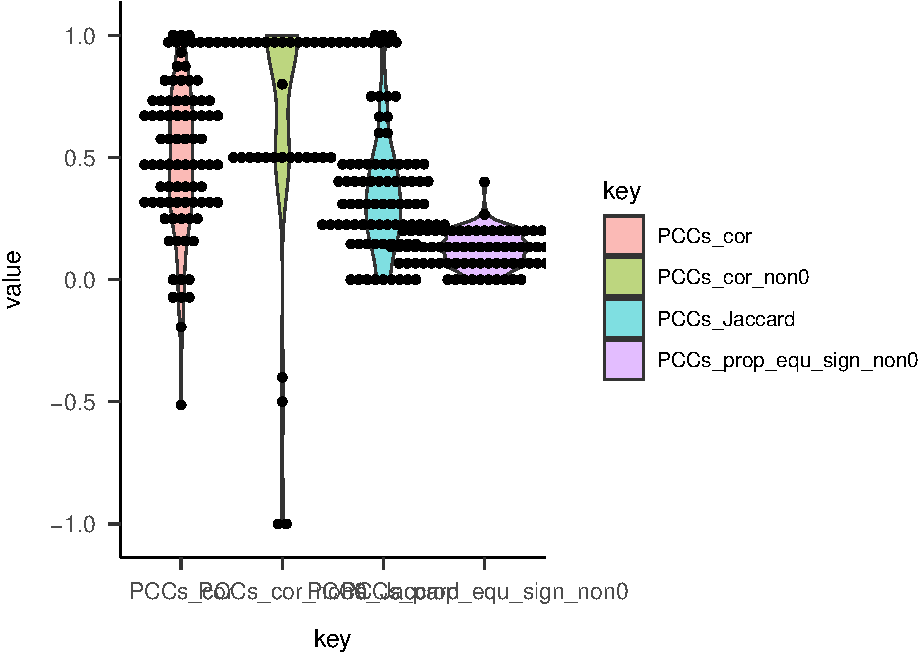
\includegraphics{ThesisAnalysisV2_files/figure-latex/comparisonsplot-1.pdf}

\hypertarget{two-examples}{%
\subsection{Two examples}\label{two-examples}}

\begin{itemize}
\tightlist
\item
  explain how were examples chosen: similar and rather small prop emtpy (both \textless{} 0.55), both only few imputed data points (less than 5 data points)
\end{itemize}

\hypertarget{low-temporal-stability-participant-53}{%
\subsubsection{Low temporal stability: Participant 53}\label{low-temporal-stability-participant-53}}

-\textgreater{} PLOT: Networks and timeseries data

\begin{itemize}
\tightlist
\item
  table with participants means, vars, demographics
\item
  explain and interpret plots
\end{itemize}

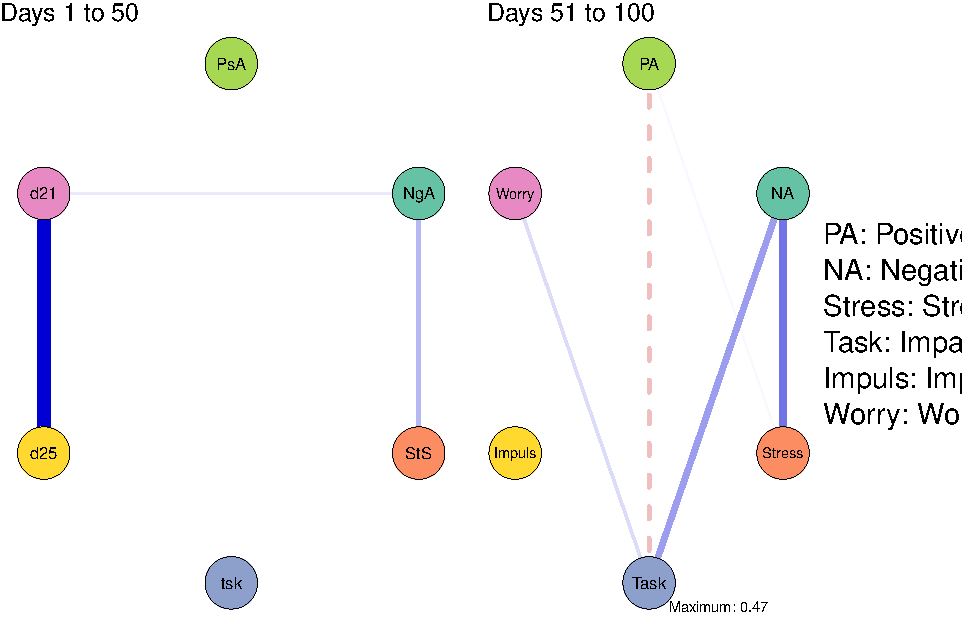
\includegraphics{ThesisAnalysisV2_files/figure-latex/plotPx53Netws-1.pdf}

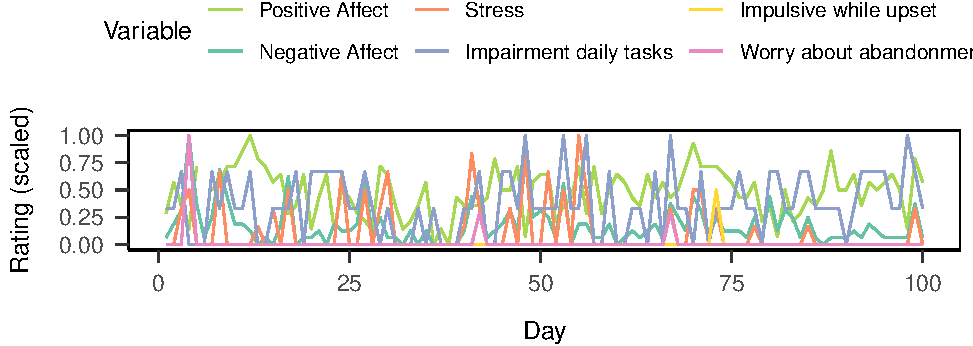
\includegraphics{ThesisAnalysisV2_files/figure-latex/plotPx53Descr-1.pdf}

\hypertarget{high-temporal-stability-participant-45}{%
\subsubsection{High temporal stability: Participant 45}\label{high-temporal-stability-participant-45}}

-\textgreater{} PLOT: Networks and timeseries data

\begin{itemize}
\tightlist
\item
  table with participants means, vars, demographics
\item
  explain and interpret plots
\end{itemize}

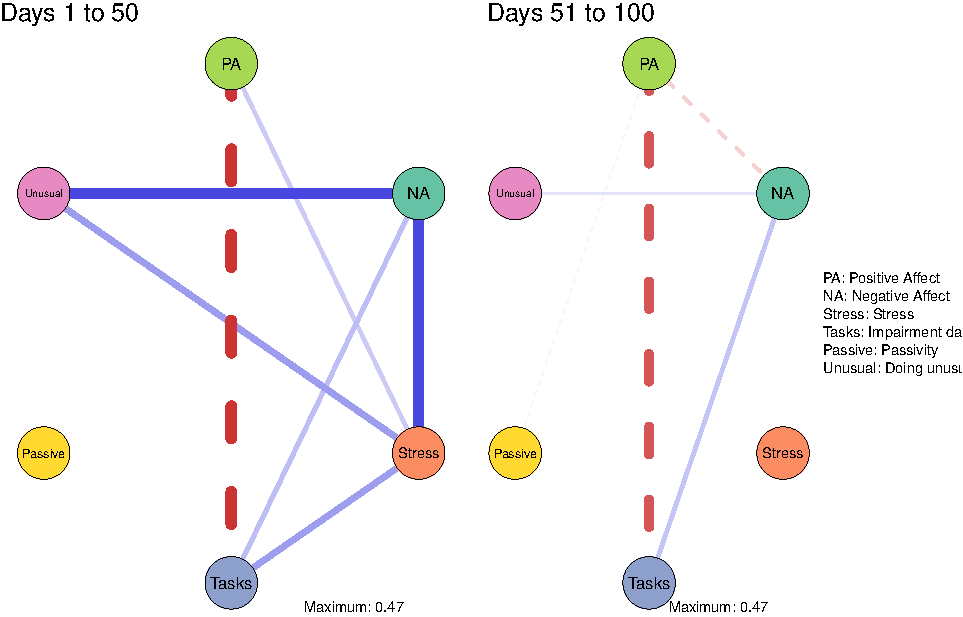
\includegraphics{ThesisAnalysisV2_files/figure-latex/plotPx45Netws-1.pdf}

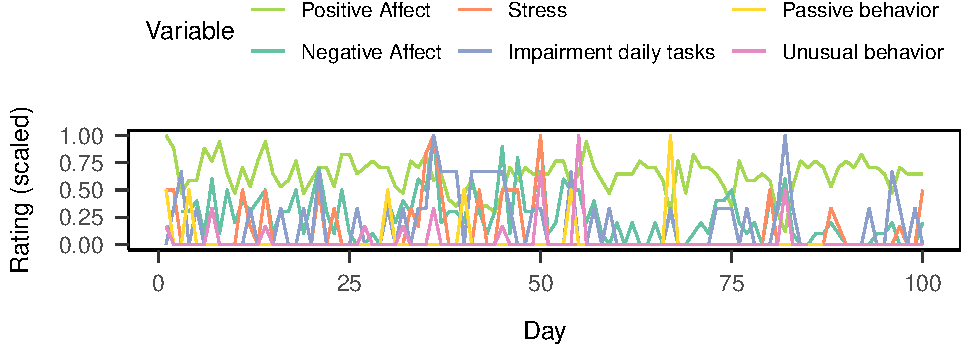
\includegraphics{ThesisAnalysisV2_files/figure-latex/plotPx45Descr-1.pdf}

\hypertarget{rq2-exploratory-regression}{%
\subsection{RQ2: Exploratory regression}\label{rq2-exploratory-regression}}

\begin{itemize}
\tightlist
\item
  table of beta estimates, R2, p as asterix, and interpretation
\end{itemize}

Call:
lm(formula = as.formula(paste0(``PCCs\_cor,'' predictors)), data = data\_merged)

Residuals:
Min 1Q Median 3Q Max
-0.85029 -0.14922 0.03142 0.20201 0.50474

Coefficients:
Estimate Standardized Std. Error t value Pr(\textgreater\textbar t\textbar)\\
(Intercept) -0.0474162 0.0000000 0.4885434 -0.097 0.9230\\
gender 0.1579527 0.2582659 0.0832580 1.897 0.0624 .
age 0.0002622 0.0128336 0.0028291 0.093 0.9265\\
recentTreatment -0.0304252 -0.1046206 0.0372450 -0.817 0.4171\\
happy 0.0173939 0.1057659 0.0255075 0.682 0.4978\\
swlsMean 0.0078294 0.0374796 0.0319544 0.245 0.8072\\
neoN 0.0178909 0.0380696 0.0847443 0.211 0.8335\\
neoE -0.1237114 -0.2585087 0.0800302 -1.546 0.1272\\
neoO 0.0337535 0.0645385 0.0697289 0.484 0.6300\\
neoA 0.0510373 0.1000355 0.0697825 0.731 0.4673\\
neoC 0.0660111 0.1670814 0.0664379 0.994 0.3242\\
nr\_imputed 0.0004862 0.0604444 0.0010226 0.475 0.6361\\
avg\_BIC -0.0003270 -0.1489720 0.0002715 -1.204 0.2329\\
PCCs\_prop\_empty 0.3334867 0.1722719 0.2455946 1.358 0.1793\\
---
Signif. codes: 0 `\emph{\textbf{' 0.001 '}' 0.01 '}' 0.05 `.' 0.1 ' ' 1

Residual standard error: 0.3017 on 63 degrees of freedom
(2 observations deleted due to missingness)
Multiple R-squared: 0.1629, Adjusted R-squared: -0.009891
F-statistic: 0.9427 on 13 and 63 DF, p-value: 0.5159

Call:
lm(formula = as.formula(paste0(``PCCs\_cor\_non0,'' predictors)),
data = data\_merged)

Residuals:
Min 1Q Median 3Q Max
-1.35817 -0.18766 0.05075 0.20287 0.57136

Coefficients:
Estimate Standardized Std. Error t value Pr(\textgreater\textbar t\textbar)\\
(Intercept) 0.4224510 0.0000000 0.9572705 0.441 0.6619\\
gender 0.0971715 0.0942475 0.1609483 0.604 0.5501\\
age -0.0112913 -0.3489184 0.0051245 -2.203 0.0347 \emph{
recentTreatment -0.2368105 -0.3854110 0.0935693 -2.531 0.0163 }
happy -0.0485086 -0.1751761 0.0481044 -1.008 0.3206\\
swlsMean 0.0379398 0.1005938 0.0705049 0.538 0.5941\\
neoN 0.0200774 0.0233946 0.1557973 0.129 0.8982\\
neoE 0.1703854 0.1738529 0.1669663 1.020 0.3149\\
neoO 0.1891781 0.2232020 0.1285100 1.472 0.1505\\
neoA -0.0327894 -0.0382882 0.1362184 -0.241 0.8113\\
neoC -0.0606645 -0.0701025 0.1593435 -0.381 0.7059\\
nr\_imputed -0.0012387 -0.0892306 0.0021273 -0.582 0.5643\\
avg\_BIC 0.0014448 0.2230158 0.0009588 1.507 0.1413\\
PCCs\_prop\_empty 0.1990008 0.0675283 0.4514714 0.441 0.6622\\
---
Signif. codes: 0 `\emph{\textbf{' 0.001 '}' 0.01 '}' 0.05 `.' 0.1 ' ' 1

Residual standard error: 0.4385 on 33 degrees of freedom
(32 observations deleted due to missingness)
Multiple R-squared: 0.4498, Adjusted R-squared: 0.2331
F-statistic: 2.075 on 13 and 33 DF, p-value: 0.04499

Call:
lm(formula = as.formula(paste0(``PCCs\_Jaccard,'' predictors)),
data = data\_merged)

Residuals:
Min 1Q Median 3Q Max
-0.46222 -0.12760 -0.01402 0.10578 0.58263

Coefficients:
Estimate Standardized Std. Error t value Pr(\textgreater\textbar t\textbar)\\
(Intercept) 0.2996337 0.0000000 0.3646266 0.822 0.4143\\
gender 0.0624267 0.1309805 0.0621269 1.005 0.3188\\
age -0.0007052 -0.0441304 0.0021096 -0.334 0.7393\\
recentTreatment -0.0419437 -0.2063487 0.0248507 -1.688 0.0963 .
happy 0.0265288 0.2062522 0.0190317 1.394 0.1682\\
swlsMean -0.0142440 -0.0884640 0.0235277 -0.605 0.5470\\
neoN -0.0711130 -0.1933963 0.0632201 -1.125 0.2649\\
neoE -0.1144637 -0.3058549 0.0596723 -1.918 0.0595 .
neoO 0.0197374 0.0482757 0.0520376 0.379 0.7057\\
neoA 0.0202703 0.0512171 0.0515861 0.393 0.6957\\
neoC 0.0451614 0.1460860 0.0493886 0.914 0.3639\\
nr\_imputed 0.0002000 0.0319740 0.0007464 0.268 0.7896\\
avg\_BIC -0.0003090 -0.1802955 0.0002021 -1.529 0.1312\\
PCCs\_prop\_empty 0.3476170 0.2316076 0.1816444 1.914 0.0601 .
---
Signif. codes: 0 `\emph{\textbf{' 0.001 '}' 0.01 '}' 0.05 `.' 0.1 ' ' 1

Residual standard error: 0.2252 on 64 degrees of freedom
(1 observation deleted due to missingness)
Multiple R-squared: 0.2263, Adjusted R-squared: 0.06911
F-statistic: 1.44 on 13 and 64 DF, p-value: 0.1663

Call:
lm(formula = as.formula(paste0(``PCCs\_prop\_equ\_sign,'' predictors)),
data = data\_merged)

Residuals:
Min 1Q Median 3Q Max
-0.132463 -0.037553 -0.003556 0.037557 0.185316

Coefficients:
Estimate Standardized Std. Error t value Pr(\textgreater\textbar t\textbar)\\
(Intercept) 2.799e-01 0.000e+00 1.063e-01 2.632 0.01061 *\\
gender 2.561e-02 9.091e-02 1.812e-02 1.413 0.16238\\
age -3.632e-05 -3.846e-03 6.151e-04 -0.059 0.95310\\
recentTreatment -8.622e-03 -7.177e-02 7.246e-03 -1.190 0.23852\\
happy 1.053e-02 1.385e-01 5.550e-03 1.897 0.06229 .\\
swlsMean -6.170e-03 -6.484e-02 6.861e-03 -0.899 0.37182\\
neoN -1.731e-02 -7.964e-02 1.843e-02 -0.939 0.35135\\
neoE -4.693e-02 -2.122e-01 1.740e-02 -2.697 0.00893 **
neoO 1.300e-02 5.379e-02 1.517e-02 0.857 0.39487\\
neoA -3.397e-03 -1.452e-02 1.504e-02 -0.226 0.82206\\
neoC 2.287e-02 1.252e-01 1.440e-02 1.588 0.11716\\
nr\_imputed 1.206e-05 3.261e-03 2.177e-04 0.055 0.95600\\
avg\_BIC -5.795e-05 -5.722e-02 5.892e-05 -0.984 0.32906\\
PCCs\_prop\_empty 7.842e-01 8.841e-01 5.297e-02 14.805 \textless{} 2e-16 ***
---
Signif. codes: 0 `\emph{\textbf{' 0.001 '}' 0.01 '}' 0.05 `.' 0.1 ' ' 1

Residual standard error: 0.06566 on 64 degrees of freedom
(1 observation deleted due to missingness)
Multiple R-squared: 0.8116, Adjusted R-squared: 0.7734
F-statistic: 21.21 on 13 and 64 DF, p-value: \textless{} 2.2e-16

Call:
lm(formula = as.formula(paste0(``PCCs\_prop\_equ\_sign\_non0,'' predictors)),
data = data\_merged)

Residuals:
Min 1Q Median 3Q Max
-0.132463 -0.037553 -0.003556 0.037557 0.185316

Coefficients:
Estimate Standardized Std. Error t value Pr(\textgreater\textbar t\textbar)\\
(Intercept) 2.799e-01 0.000e+00 1.063e-01 2.632 0.010614 *\\
gender 2.561e-02 1.655e-01 1.812e-02 1.413 0.162376\\
age -3.632e-05 -7.000e-03 6.151e-04 -0.059 0.953099\\
recentTreatment -8.622e-03 -1.306e-01 7.246e-03 -1.190 0.238518\\
happy 1.053e-02 2.521e-01 5.550e-03 1.897 0.062292 .\\
swlsMean -6.170e-03 -1.180e-01 6.861e-03 -0.899 0.371820\\
neoN -1.731e-02 -1.450e-01 1.843e-02 -0.939 0.351348\\
neoE -4.693e-02 -3.862e-01 1.740e-02 -2.697 0.008928 **
neoO 1.300e-02 9.791e-02 1.517e-02 0.857 0.394875\\
neoA -3.397e-03 -2.643e-02 1.504e-02 -0.226 0.822063\\
neoC 2.287e-02 2.279e-01 1.440e-02 1.588 0.117162\\
nr\_imputed 1.206e-05 5.935e-03 2.177e-04 0.055 0.955999\\
avg\_BIC -5.795e-05 -1.041e-01 5.892e-05 -0.984 0.329058\\
PCCs\_prop\_empty -2.158e-01 -4.429e-01 5.297e-02 -4.075 0.000129 ***
---
Signif. codes: 0 `\emph{\textbf{' 0.001 '}' 0.01 '}' 0.05 `.' 0.1 ' ' 1

Residual standard error: 0.06566 on 64 degrees of freedom
(1 observation deleted due to missingness)
Multiple R-squared: 0.376, Adjusted R-squared: 0.2493
F-statistic: 2.967 on 13 and 64 DF, p-value: 0.001934

\hypertarget{discussion}{%
\section{Discussion}\label{discussion}}

\hypertarget{temporal-stability-of-idiographic-networks}{%
\subsection{Temporal Stability of Idiographic networks}\label{temporal-stability-of-idiographic-networks}}

\hypertarget{implications}{%
\subsubsection{Implications}\label{implications}}

\begin{itemize}
\item
  \emph{assuming that change scores indeed reflect change in data generating process}
\item
  lack of stability poses challenge to idiographic models as useful representation that generalize within an individual, stationarity assumption and power problems, potential solutions are being developed and needed (multilevel estimation, baysian, timevarying var)
\item
  implications for power: depending on process of interest, we may lose or gain power depending on T
\item
  high stability: great, stationarity realistic, gives us more slack in research design (not lose power when extedning measurmeent period?)
\item
  bet is on dynamics of system, so change itself is of interest.
  EWS etc\ldots{}
\item
  relate to idea of monitoring change, critical slowing down, phase transitions, ROM
\item
  Variability seems to be a thing
\end{itemize}

\hypertarget{possibles-explanations}{%
\subsubsection{Possibles explanations}\label{possibles-explanations}}

\begin{itemize}
\tightlist
\item
  intra-individual variation: changes in network structure may be related to factors related to the individual (eg traits, circumstances, quality of the data, response style\ldots{} provide list), should be addressed in future study designs
\item
  Measurement error
\item
  Important assumption made by (idiographic) network models is that constructs were measured without error. Little published research on this, but eg. SchreuderEtAl2020 assessed participants interpretation of EMA items over the course of 6 months and concluded interpretation was consistent. Changes in item interpretation also known as measurement invariance or response shift bias. (the other study cited in lauras review)
\item
  Conscientiousness? Response style?
\item
  stabilitiy as a trait?
\end{itemize}

\hypertarget{strengths-of-the-current-study}{%
\subsection{Strengths of the current study}\label{strengths-of-the-current-study}}

\begin{itemize}
\tightlist
\item
  some major features made data a good candidate
\item
  daily lags equal (opposed to designs using several per day)
\item
  consecutive periods where no change should be expected (eg no therapy or intervention etc)
\end{itemize}

\hypertarget{limitations-of-the-current-study}{%
\subsection{Limitations of the current study}\label{limitations-of-the-current-study}}

\hypertarget{power}{%
\subsubsection{Power}\label{power}}

\begin{itemize}
\tightlist
\item
  heterogeneous sample, low power
\item
  noisy data:
\item
  Kalman imputation assumes MCAR, but likely there is some bias.
\item
  sources of noise: Imputation, Missingness, MARS,, detrending, Measurement error, sample size
\item
  regression underpowered
\end{itemize}

\hypertarget{constraints-to-generalizability}{%
\subsubsection{Constraints to generalizability}\label{constraints-to-generalizability}}

\begin{itemize}
\tightlist
\item
  exploratory work, needs replication
\item
  how representive is data for current ESM designs?
\item
  Other network methods?
\item
  modeling decisions?
\item
  conceptualization of model similarity / stability. We focus on similarity of global network structure, but there are many more ways to describe and interpret networks which may or may not be relevant for replicability: network comparison test, predictive networks models, sensitivity and specificity of recovered edges if true network known
\end{itemize}

\hypertarget{future-directions}{%
\subsection{Future directions}\label{future-directions}}

\hypertarget{idiographic-network-models}{%
\subsubsection{Idiographic network models}\label{idiographic-network-models}}

\begin{itemize}
\tightlist
\item
  bootstrapping etc for idiographic applications?
\item
  measurement error
\item
  lasso regularization: empty edge deos not actually imply independence
\item
  discussion on centrality measures and problems with those and their interpretation
\item
  how to conceptualize replicability, stability, reproducibility
\item
  time varying VAR
\item
  simulation studies on effects of modeling decisions: variable transformations, detrending, missing data imputation, missing data mechanisms
\end{itemize}

\hypertarget{network-theory}{%
\subsubsection{Network theory}\label{network-theory}}

\begin{itemize}
\tightlist
\item
  stationarity versus temporal stability and complex dynamics
\item
  empirical work on: missing data mechanism
\item
  more theoretical groundwork: what kind of things are networks made of? what things to include in the network? What variable properties are desireable, what levels of clustering is desirable?
\item
  is a partial correlation a clinically useful concept? (feasibility study)
\item
  what model features are a useful metric?
\item
  which (changes in) features have clinical relevance, which may be neglected?
\item
  EWS as the way forward?
\item
  formal case conceptualizations?
\item
  how do we expect processes to vary? eg, linear trend is not possible bec range is bound, so extrapolation not possible and detrending necessarily biased by time range measured
\item
  oscillation / sine wave? what amplitude and phase?
\end{itemize}

\hypertarget{conclusion}{%
\section{Conclusion}\label{conclusion}}

\begin{itemize}
\tightlist
\item
  warrants caution regarding the inferences we draw from idio netw right now, as some would lead to very different interpretations
\item
  not well understood why this is the case, whether it's measurement error, item distribution,
\item
  it's more a momentary impression of item correlations in certain period of time
\item
  stability of process which extends beyond this period and should eg inform interventions needs more work
\end{itemize}

\newpage

\hypertarget{references}{%
\section{References}\label{references}}

\begingroup
\setlength{\parindent}{-0.5in}
\setlength{\leftskip}{0.5in}

\hypertarget{refs}{}
\begin{CSLReferences}{1}{0}
\leavevmode\hypertarget{ref-BeckJackson2020a}{}%
Beck, Emorie D., \& Jackson, J. J. (2020). Consistency and change in idiographic personality: A longitudinal ESM network study. \emph{Journal of Personality and Social Psychology}, \emph{118}(5), 1080--1100. \url{https://doi.org/10.1037/pspp0000249}

\leavevmode\hypertarget{ref-BeckJackson2021}{}%
Beck, Emorie D., \& Jackson, J. J. (2021). Idiographic personality coherence: A quasi experimental longitudinal ESM study. \emph{European Journal of Personality}, 08902070211017746. \url{https://doi.org/10.1177/08902070211017746}

\leavevmode\hypertarget{ref-BorsboomCramer2013}{}%
Borsboom, D., \& Cramer, A. O. J. (2013). Network analysis: An integrative approach to the structure of psychopathology. \emph{Annual Review of Clinical Psychology}, \emph{9}(1), 91--121. \url{https://doi.org/10.1146/annurev-clinpsy-050212-185608}

\leavevmode\hypertarget{ref-BurgerEtAl2020}{}%
Burger, J., Veen, D. C. van der, Robinaugh, D. J., Quax, R., Riese, H., Schoevers, R. A., \& Epskamp, S. (2020). Bridging the gap between complexity science and clinical practice by formalizing idiographic theories: A computational model of functional analysis. \emph{BMC Medicine}, \emph{18}(1), 99. \url{https://doi.org/10.1186/s12916-020-01558-1}

\leavevmode\hypertarget{ref-CavigliaColeman2016}{}%
Caviglia, G., \& Coleman, N. (2016). Idiographic network visualizations. \emph{Leonardo}, \emph{49}(5), 447--447. \url{https://doi.org/10.1162/LEON_a_01267}

\leavevmode\hypertarget{ref-CramerEtAl2010}{}%
Cramer, A. O. J., Waldorp, L. J., Maas, H. L. J. van der, \& Borsboom, D. (2010). Comorbidity: A network perspective. \emph{Behavioral and Brain Sciences}, \emph{33}(2-3), 137--150. \url{https://doi.org/10.1017/S0140525X09991567}

\leavevmode\hypertarget{ref-EpskampEtAl2018}{}%
Epskamp, S., Borsboom, D., \& Fried, E. I. (2018). Estimating psychological networks and their accuracy: A tutorial paper. \emph{Behavior Research Methods}, \emph{50}(1), 195--212. \url{https://doi.org/10.3758/s13428-017-0862-1}

\leavevmode\hypertarget{ref-EpskampEtAl2018a}{}%
Epskamp, S., van Borkulo, C. D., van der Veen, D. C., Servaas, M. N., Isvoranu, A.-M., Riese, H., \& Cramer, A. O. J. (2018). Personalized Network Modeling in Psychopathology: The Importance of Contemporaneous and Temporal Connections. \emph{Clinical Psychological Science}, \emph{6}(3), 416--427. \url{https://doi.org/10.1177/2167702617744325}

\leavevmode\hypertarget{ref-EpskampEtAl2018b}{}%
Epskamp, S., Waldorp, L. J., Mõttus, R., \& Borsboom, D. (2018). The gaussian graphical model in cross-sectional and time-series data. \emph{Multivariate Behavioral Research}, \emph{53}(4), 453--480. \url{https://doi.org/10.1080/00273171.2018.1454823}

\leavevmode\hypertarget{ref-FrumkinEtAl2020}{}%
Frumkin, M. R., Piccirillo, M. L., Beck, E. D., Grossman, J. T., \& Rodebaugh, T. L. (2020). Feasibility and utility of idiographic models in the clinic: A pilot study. \emph{Psychotherapy Research}, \emph{0}(0), 1--15. \url{https://doi.org/10.1080/10503307.2020.1805133}

\leavevmode\hypertarget{ref-GeEtAl2019}{}%
Ge, F., Yuan, M., Li, Y., Zhang, J., \& Zhang, W. (2019). Changes in the network structure of posttraumatic stress disorder symptoms at different time points among youth survivors: A network analysis. \emph{Journal of Affective Disorders}, \emph{259}, 288--295. \url{https://doi.org/10.1016/j.jad.2019.08.065}

\leavevmode\hypertarget{ref-Harvey1989}{}%
Harvey, A. C. (1989). \emph{Forecasting, Structural Time Series Models and the Kalman Filter}. Cambridge University Press.

\leavevmode\hypertarget{ref-HoffartJohnson2020}{}%
Hoffart, A., \& Johnson, S. U. (2020). Within-person networks of clinical features of social anxiety disorder during cognitive and interpersonal therapy. \emph{Journal of Anxiety Disorders}, \emph{76}, 102312. \url{https://doi.org/10.1016/j.janxdis.2020.102312}

\leavevmode\hypertarget{ref-HoweEtAl2020}{}%
Howe, E., Bosley, H. G., \& Fisher, A. J. (2020). Idiographic network analysis of discrete mood states prior to treatment. \emph{Counselling and Psychotherapy Research}, \emph{20}(3), 470--478. https://doi.org/\url{https://doi.org/10.1002/capr.12295}

\leavevmode\hypertarget{ref-KuranovaEtAl2020}{}%
Kuranova, A., Booij, S. H., Menne-Lothmann, C., Decoster, J., Winkel, R. van, Delespaul, P., \ldots{} al., et. (2020). Measuring resilience prospectively as the speed of affect recovery in daily life: A complex systems perspective on mental health. \emph{BMC Medicine}, \emph{18}(1), 36. \url{https://doi.org/10.1186/s12916-020-1500-9}

\leavevmode\hypertarget{ref-MansuetoEtAl2020}{}%
Mansueto, A. C., Wiers, R., van Weert, J., Schouten, B. C., \& Epskamp, S. (2020). \emph{Investigating the Feasibility of Idiographic Network Models}. Retrieved from \url{https://osf.io/hgcz6}

\leavevmode\hypertarget{ref-Molenaar2004}{}%
Molenaar, P. C. M. (2004). A manifesto on psychology as idiographic science: Bringing the person back into scientific psychology, this time forever. \emph{Measurement: Interdisciplinary Research \& Perspective}, \emph{2}(4), 201--218. \url{https://doi.org/10.1207/s15366359mea0204_1}

\leavevmode\hypertarget{ref-ScholtenEtAl2020}{}%
Scholten, S., Lischetzke, T., \& Glombiewski, J. (2020). \emph{Toward data-based case conceptualization: A functional analysis approach with ecological momentary assessment}. PsyArXiv. \url{https://doi.org/10.31234/osf.io/prg7n}

\leavevmode\hypertarget{ref-SegalEtAl2020}{}%
Segal, A., Wald, I., Lubin, G., Fruchter, E., Ginat, K., Ben Yehuda, A., \ldots{} Bar-Haim, Y. (2020). Changes in the dynamic network structure of PTSD symptoms pre-to-post combat. \emph{Psychological Medicine}, \emph{50}(5), 746--753. \url{https://doi.org/10.1017/S0033291719000539}

\leavevmode\hypertarget{ref-ShapiroWilk1965}{}%
Shapiro, S. S., \& Wilk, M. B. (1965). An analysis of variance test for normality (complete samples). \emph{Biometrika}, \emph{52}(3/4), 591--611. \url{https://doi.org/10.2307/2333709}

\leavevmode\hypertarget{ref-vonStockertEtAl2018}{}%
Stockert, S. H. H. von, Fried, E. I., Armour, C., \& Pietrzak, R. H. (2018). Evaluating the stability of DSM-5 PTSD symptom network structure in a national sample of u.s. Military veterans. \emph{Journal of Affective Disorders}, \emph{229}, 63--68. \url{https://doi.org/10.1016/j.jad.2017.12.043}

\leavevmode\hypertarget{ref-ThononEtAl2020}{}%
Thonon, B., Van Aubel, E., Lafit, G., Della Libera, C., \& Larøi, F. (2020). Idiographic analyses of motivation and related processes in participants with schizophrenia following a therapeutic intervention for negative symptoms. \emph{BMC Psychiatry}, \emph{20}(1), 464. \url{https://doi.org/10.1186/s12888-020-02824-5}

\leavevmode\hypertarget{ref-WichersEtAl2016}{}%
Wichers, M., Groot, P. C., \& Psychosystems, E. G., ESM Group. (2016). Critical slowing down as a personalized early warning signal for depression. \emph{Psychotherapy and Psychosomatics}, \emph{85}(2), 114--116. \url{https://doi.org/10.1159/000441458}

\leavevmode\hypertarget{ref-WrightEtAl2015a}{}%
Wright, Aidan G. C., Beltz, A. M., Gates, K. M., Molenaar, P. C. M., \& Simms, L. J. (2015). Examining the dynamic structure of daily internalizing and externalizing behavior at multiple levels of analysis. \emph{Frontiers in Psychology}, \emph{6}. \url{https://doi.org/10.3389/fpsyg.2015.01914}

\leavevmode\hypertarget{ref-WrightEtAl2015}{}%
Wright, Aidan G. C., Hopwood, C. J., \& Simms, L. J. (2015). Daily interpersonal and affective dynamics in personality disorder. \emph{Journal of Personality Disorders}, \emph{29}(4), 503--525. \url{https://doi.org/10.1521/pedi.2015.29.4.503}

\leavevmode\hypertarget{ref-WrightSimms}{}%
Wright, Aidan G. C., \& Simms, L. J. (n.d.). \emph{Stability and fluctuation of personality disorder features in daily life}. 16.

\leavevmode\hypertarget{ref-YaziciYolacan2007}{}%
Yazici, B., \& Yolacan, S. (2007). A comparison of various tests of normality. \emph{Journal of Statistical Computation and Simulation}, \emph{77}(2), 175--183. \url{https://doi.org/10.1080/10629360600678310}

\end{CSLReferences}

\endgroup


\clearpage
\renewcommand{\listfigurename}{Figure captions}

\clearpage
\renewcommand{\listtablename}{Table captions}


\end{document}
